\documentclass{article}
\usepackage{xcolor}
\usepackage{textcomp}
\usepackage{hyperref}
\usepackage{graphicx}

% relative path to images directory
% \graphicspath{ {./images/} }

\title{Research of Parameters in Strategies of the Iterated Continuous Prisoner's Dilemma}
\author{Adrian Hossner}
\date{ } % display no date

\begin{document}
\maketitle

\newpage
\tableofcontents
\newpage

\section*{Abstract}

\section{Introduction}

\begin{itemize}

	% Key idea:
	% Much uncertainty spread out because of (far-)right populists.
	% With insecurity comes random behaviour.
	% This simulations shows the difference of a random and a determined strategy.

	\item Interactions\\
		implication range is wide:\\
		from two persons in a relationship to countries in alliance\\
		from two impala's algrooming to zebras warning the herd about a lion \\
	% https://www.cell.com/trends/ecology-evolution/pdf/S0169-5347(00)88988-0.pdf

	\item Key hook:\\
		helping someone with possible cost -- cooperation\\
		being selfish but breaking trust -- defection\\

	\item model PD:\\
		single interaction\\
		already well analysed\\
		Nash found solution/equilibrium\\

	\item Iterated:\\
		more interesting, insightful\\
		strategies\\

	\item non-suited variants:\\
		Axelrod's Tournament\\
		Evolution\\

	\item continuous:\\
		more complex, accurate\\

	\item parameters:\\
		determines behaviour\\
		create surface\\
		the part that has not been experimented\\

	\item overall and difference:\\
		overall: wealth of population\\
		difference: competence between individuals\\

\end{itemize}

\section{Theoretical Foundations}
\begin{itemize}

	\item Game Theory (optional, not needed for understanding)\\
		mathematical framework to investigate interactions\\

	\item Prisoner's Dilemma:\\
		
The Prisoner's Dilemma (PD) is a famous intellectual game in Game Theory. 
It was invented by Merrill Flood and Melvin Dresher in 1950. 
In order to understand the dilemma, a proper context has to be established. 
Two persons are arrested and are sued for having stolen something. 
The police, however, has not enough evidence to imprison them. 
As a consequence of that, the police interrogates the two criminals. 
They can either say nothing or confess that the other suspect was involved in the crime. 
They can either cooperate or defect without having the possibility to talk to each other before the decision. 
A certain tactic is being used by the police officers. 
They make it profitable for the criminals to confess. 
They let the criminal out of prison earlier if he/she confesses. 
But if the other also confesses, both stay long in prison. 
If he/she says nothing and the other confesses, he/she will stay very long in prison. 
If, however, both stay silent, both of them go to prison in a relatively short amount of time. 
The following matrix visualises the pay-off's in this game in a comprehensive way:

% specific pay-off matrix
\begin{center}
\begin{tabular}{ c|c|c }
   & C & D \\ 
   \hline
 C & 3, 3 & 10, 0\\  
   \hline
 D & 0, 10 & 5, 5
\end{tabular}
\end{center}

C stands for cooperation and D stands for defection. 
Cooperation is defined by remaining silent whereas defection means confessing. 
The dilemma consists of the following. 
Confessing seems attractive since the interrogated criminal can walk out freely without going to prison. 
However, if the second criminal also confesses, both get five years in prison. 
This is, nevertheless, the worst outcome for both which could have been avoided as both could have stayed silent.\\
John Nash, a mathematician which made great contributions in Game Theory, has proved that it is the most logical option for both to confess, always. 
A Nash-equilibrium is introduced. 
It defines a stable state in which both would not change their decision even though they would know if the other cooperated or defected.\\
This game composes a one-time interaction very well in a mathematical and analytical perspective. 
The pay-off's in the matrix can be changed as long as these rules stay fulfilled.
% \url{https://www.investopedia.com/terms/n/nash-equilibrium.asp}

% general pay-off matrix
\begin{center}
\begin{tabular}{ c|c|c }
   & C & D \\ 
   \hline
 C & R, R & S, T\\  
   \hline
 D & T, S & P, P
\end{tabular}
\end{center}

$$T > R > P > S$$

	\item Iterated:\\
		
The Iterated Prisoner's Dilemma (IPD) is a game which extends the PD. 
As the name suggests, the PD is played a number of times sequentially. 
After each round the pay-off gets accumulated to the points one strategy has already gained. 
A strategy is to be considered as an autonomous player which has its own behaviour.
A strategy has the whole history of its own contributions and the ones of the opponent at hand to generate the decision for the next round.
These decisions are calculated by using conditions and probabilities that will be applied on the given data.
In this, and in the following variants, the analogy to the real world is changed.
It is wanted to maximize their output in the end.
In contrary to the initial variant, it means that high number are wanted instead of unwanted.
To still hold on the idea of the Prisoner's Dilemma, the pay-off's could be interpreted as to be subtracted.
Meaning, the bigger the points, the sooner one gets out of prison.
Since a strategy wants to gain as many points as possible, the pay-off matrix should be altered accordingly.\\

\begin{center}
\begin{tabular}{ c|c|c }
   & C & D \\ 
   \hline
 C & 3, 3 & 0, 5\\  
   \hline
 D & 5, 0 & 1, 1
\end{tabular}
\end{center}

And to generalise this matrix as well, the numbers can be replaced with variables.
These variables $T, R, P \: \mathrm{and} \: T$ % can be changes no matter how ...


\begin{center}
\begin{tabular}{ c|c|c }
   & C & D \\ 
   \hline
 C & R, R & S, T\\  
   \hline
 D & T, S & P, P
\end{tabular}
\end{center}

$$T < R < P < S$$
$$2R > T + S$$

The Nash-equilibrium in the IPD differs from that in the PD.
This means that cooperation can earn out long-term. 
By cooperating, one is building trust with another. 
One strategy can only get the maximum points, which can be gained by always getting the 5 points each round, by defecting and the opponent's cooperation. 
Since the opponent will likely not cooperate after one strategy always defects, the maximum is practically impossible to receive. 
So, the relative high amount and the possibility of getting it for both is by cooperating.\\
The number of round that will be played has to be unknown to both strategies. 
There is no sense in cooperating the last round since trust does not matter after the game is ended. 
And because trust will be given up in the last round, there is no sense for both to keep trust the second last round. 
This will end up in an inductive defection behaviour for both strategies the whole game.\\
This extension of the PD allows us to simulate a relationship over time where the two players interact multiple times.

	\item Continuous:\\

The continuous variant is considered more accurate to the real world since the decisions are rather rare only either cooperation or defection.
The amount of cooperation is called investment and can range from zero to one (0 to 1) where full defection is represented by 0 and cooperation corresponds to 1.
One would suspect a very similar pay-off system to the iterated variant.
In the discrete version, it looked like this:

\begin{center}
\begin{tabular}{ c c }
Pay-off Player A & Pay-off Player B\\
\begin{tabular}{ c|c|c }
   & $C_A$ & $D_A$ \\ 
   \hline
 $C_B$ & 3 & 5\\  
   \hline
 $D_B$ & 0 & 1
\end{tabular}
&
\begin{tabular}{ c|c|c }
   & $C_A$ & $D_A$ \\ 
   \hline
 $C_B$ & 3 & 0\\  
   \hline
 $D_B$ & 5 & 1
\end{tabular}
\end{tabular}
\end{center}

This is possible by bilinearly interpolating the pay-off matrix so that the lines become fluid.
This will establish a field that can be represented by colour grades, a heat map.
The equation for utilizing this heat map correctly are also displayed.

% TODO: 
% - include ChatGPT in paper (say that I used it to generate the figures)
% - ask ChatGPT to make replace numbers with variables (T, R, P, S) to generalise
% - display the functions ChatGPT used to generate the heat maps
% - write a fluid transit from bilinear interpolated to equations
\begin{figure}[htbp]
	\centering
	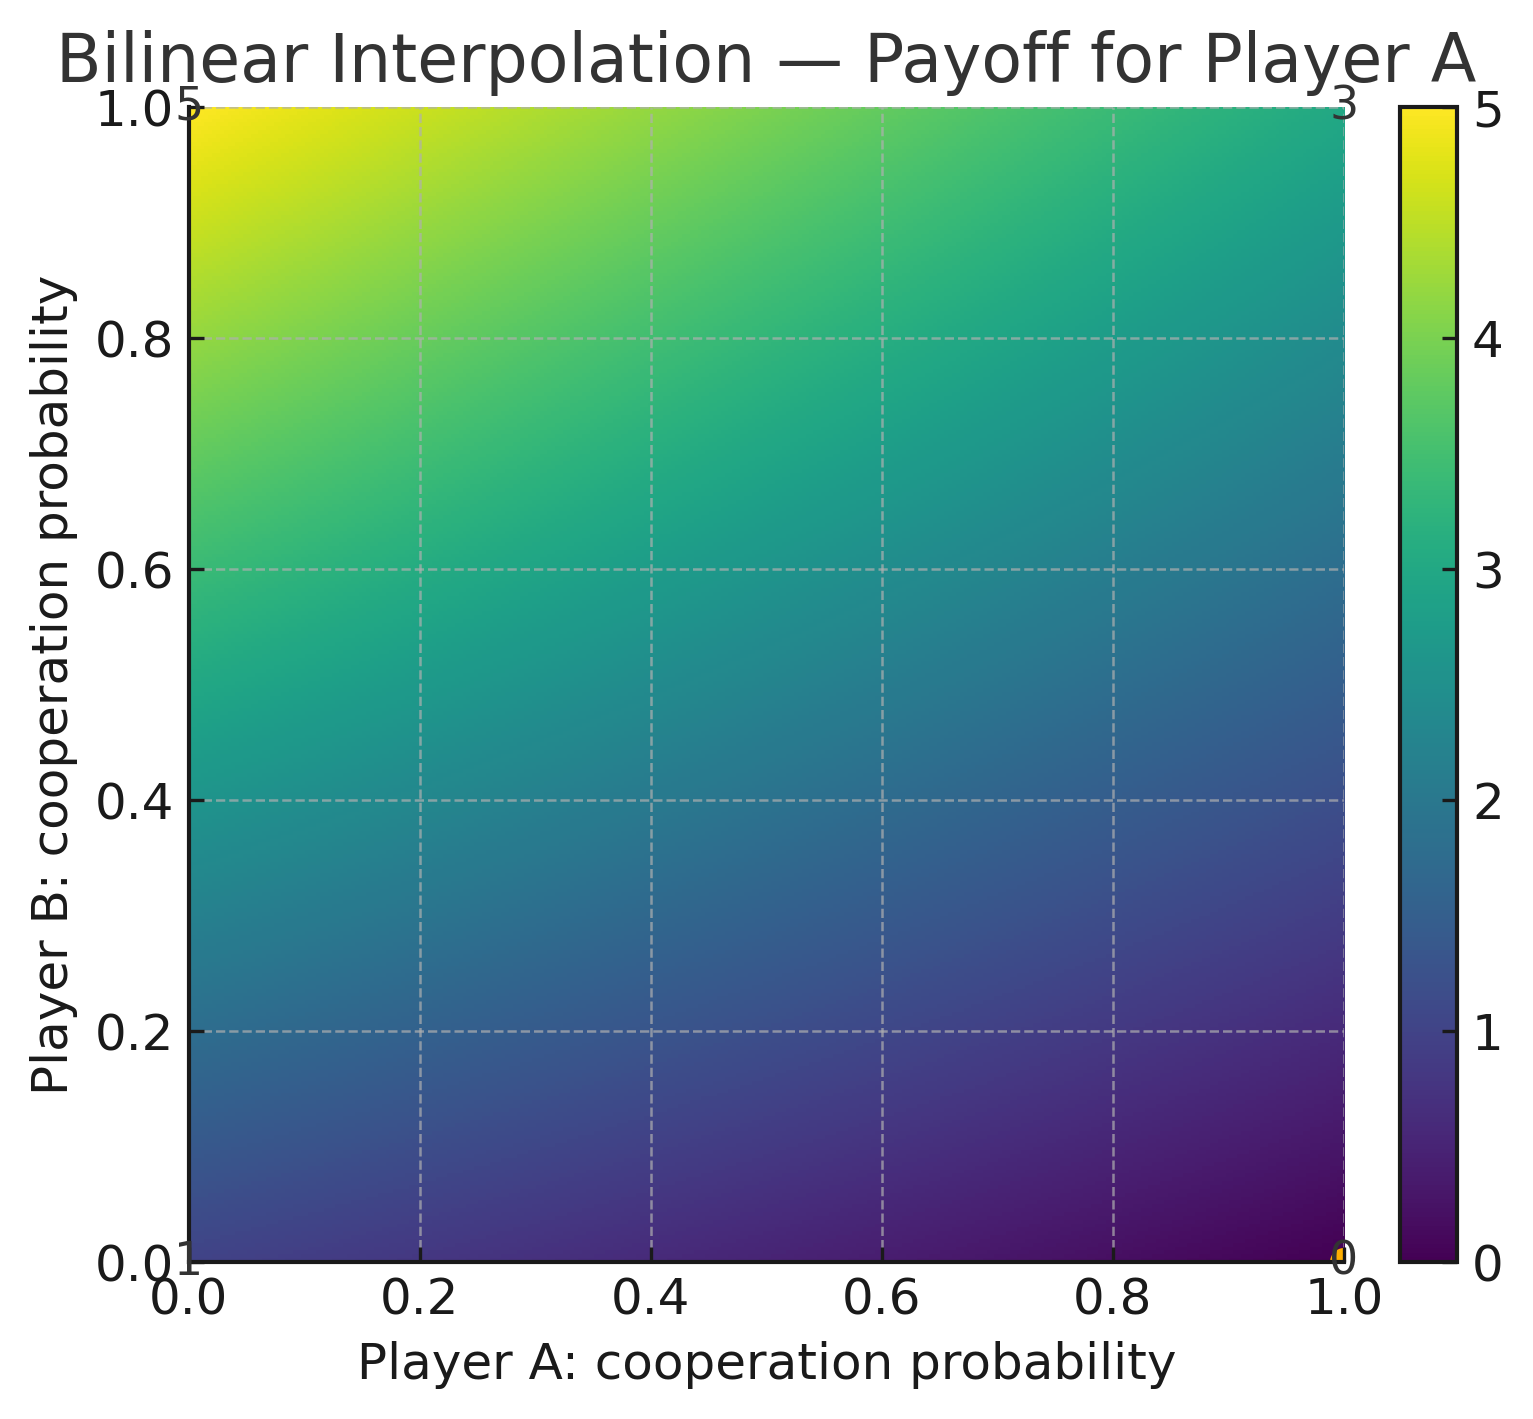
\includegraphics[width=0.45\textwidth]{images/pd_heatmap_A}\hfill
	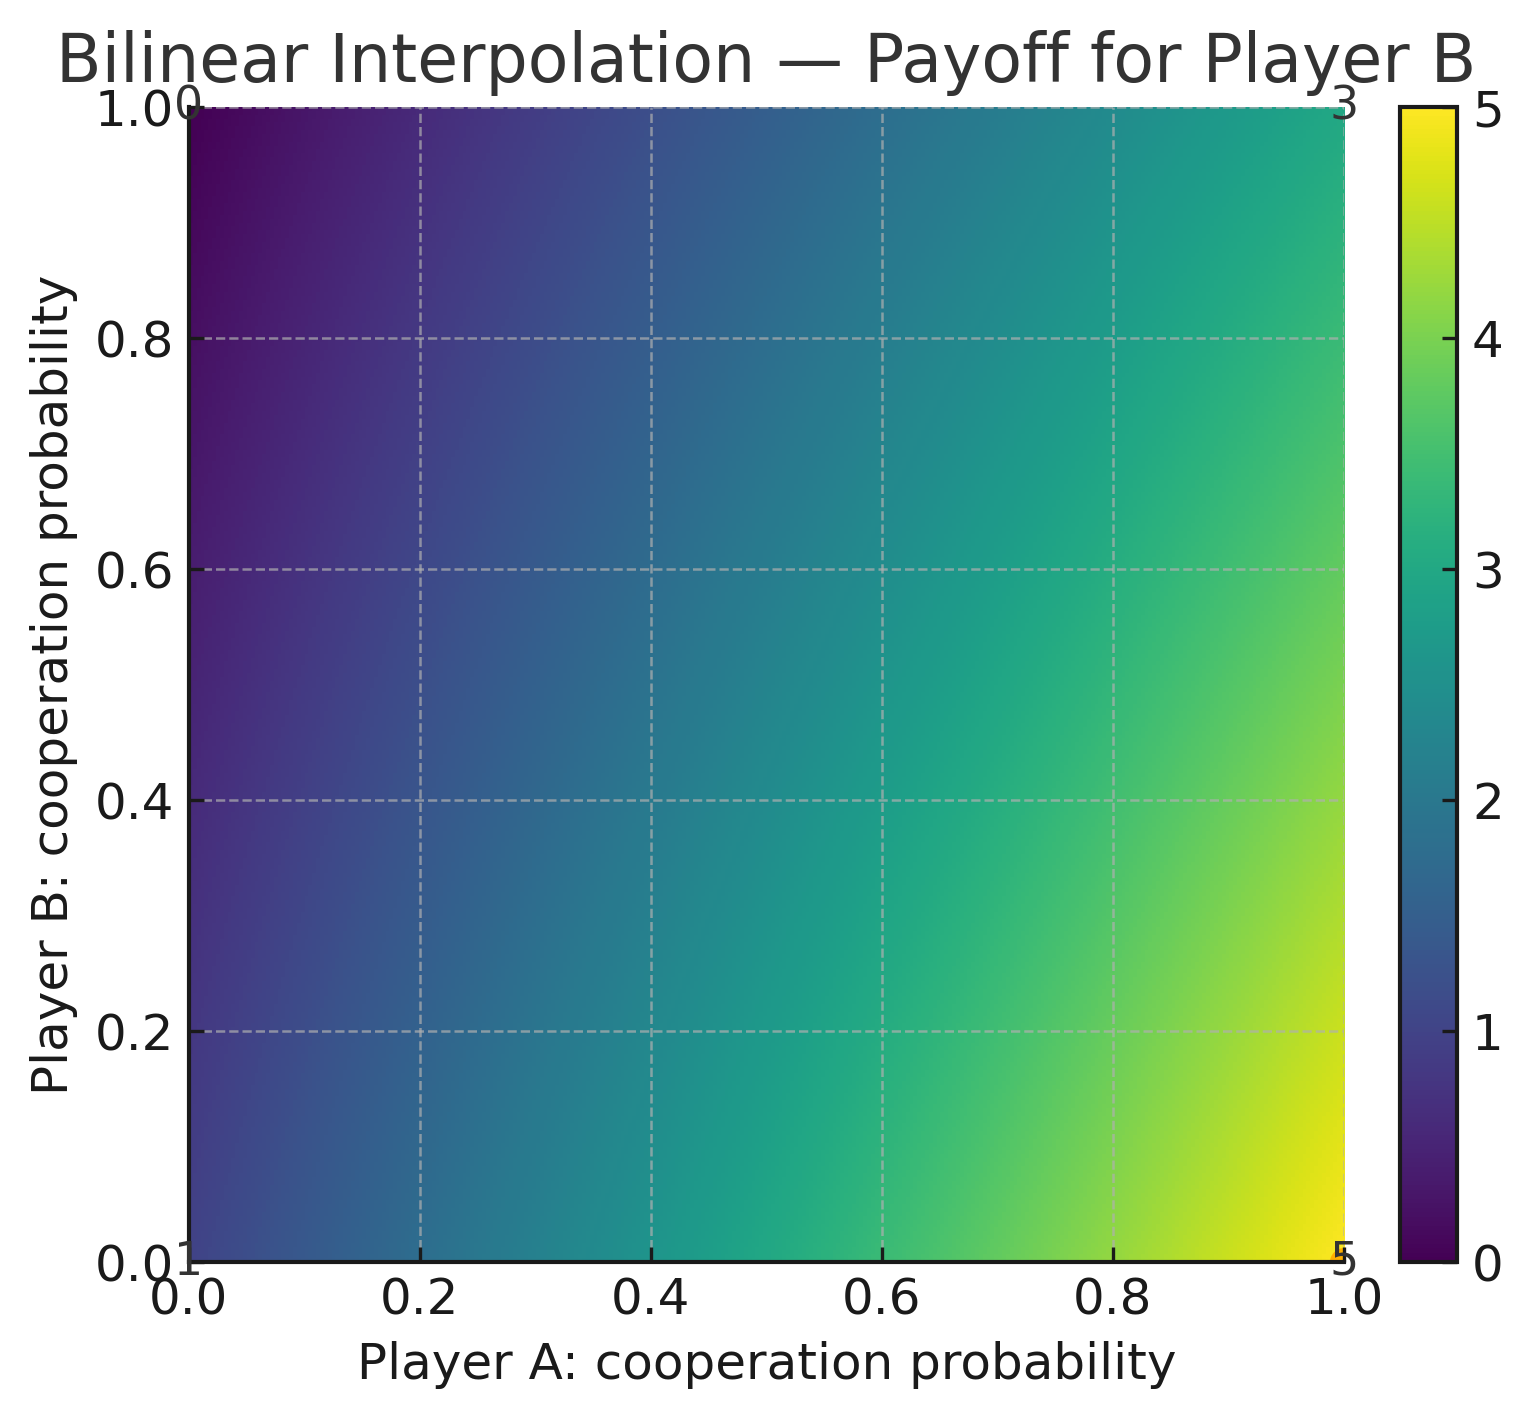
\includegraphics[width=0.45\textwidth]{images/pd_heatmap_B}
	\caption{Pay-off hash maps in the continuous variant of the IPD.}
\end{figure}

I used ChatGPT-o4 to generate these heat maps.
It generated them using these functions:

$$U_A = (1-x)(1-y)R_A + (1-x)yS_A + x(1-y)T_A + xyP_A$$
$$U_B = (1-x)(1-y)R_B + (1-x)yS_B + x(1-y)T_B + xyP_B$$

These functions are applied to every point on the map.
The variable x is the investment of strategy A and y is the investment of strategy B.
There is, however, another way of determine the pay-off's.
This approach uses only equations instead.
It is much easier to implement but understanding is the difficult part.
This pay-off system of [sciencedirect.com] is formed by:

$$P_A = y - c*x$$
$$P_B = x - c*y$$

$P_A$ and $P_B$ are the pay-off's of strategy A and B respectively.
The coefficient c ranges, as well as x and y, from 0 to 1 and describes the cost-to-benefit ratio.
The base of the pay-off's are the opponent's investment.
Then the strategy's own investment gets multiplied by the coefficient c and then is subtracted from the base.
This means the pay-off is highly influenced by the opponent's investment.
Let's see if the principles of the initial PD are still valid.
It is better for one to defect (submit a 0) to get rid of the subtraction.
And it is better for the strategy if the opponent's cooperates.
If both defect, one gets zero points.
If both cooperate, both get $1 - c$ points.
If, however, one strategy exploits the opponent, meaning it defects while the other cooperates, it will get the maximum points being 1.
The opponent would then get $-c$ points.
This is the least one can receive.
[Examples of coefficient c]
\\

		% 0 to 1 rather than cooperation or defection\\
		% Pay-off system\\ % https://www.sciencedirect.com/science/article/pii/S0022519306004255?casa_token=hIA0lYvzjf8AAAAA:Up2uQ89wotaLz7s1R0dM2FK7SaulAo40wIM-BdM9yooZ8uJeRL6mPs-K55dPNGs4XkcclNVjDQ#aep-section-id24
		% more accurate\\
		% more complex, generates more data \textrightarrow more insightful\\

	\item Noise:\\

Noise in the ICPD is the equivalent to miscommunication or misunderstanding in the real world.
In this variant of the PD, noise is essential to trigger interesting outcomes.
When a game of the ICPD is started and two strategies who start with a full investment, many strategies only respond with full investments.
So noise is necessary to trigger continuous investments. 
Without noise, in many cases, the ICPD would be equivalent to the IPD.

		% sometimes necessary to trigger continuous investments\\
		% simulates misunderstandings\\

	\item Simultaneous vs Alternating:\\

Two main differences can be seen when simulating an iterated variant of the PD.
On one hand there is the simultaneous form whereby the strategies submit their contribution at the same time.
On the other hand, there is the alternating form in which on e strategy submits its contribution and the other strategy can respond to this contribution is that round.
Since the alternating form gives and advantage to the strategy which is allowed to respond, this only makes things more complicated than necessary.
So, this analysis is only dedicated to the simultaneous form.

	\item Current Findings:\\

In the simpler variants, e.g. the IPD without noise, it has been proved many times over that the strategy Tit-For-Tat is the most successful one. [sources]
The success of strategies, however, can vary depending on certain conditions such as the influence of noise or different pay-off systems where continuous investments can be submitted.
So, the very specific area of the simultaneous ICPD, has not been very well explored.
...

		% (None really)\\
		% Not well explored: simultaneous Iterated Continuous Prisoner's Dilemma

\end{itemize}

\section{Methods and Implementation}
\begin{itemize}

	\item Parameter-based:\\

The main idea of this paper is to use parameter-based strategies.
These strategies hold a parameter that defines the behaviour of the strategy.
The parameter will always range from 1 to 10 inclusively.
[Example]


		% Define parameter within strategies\\
		% determine the behaviour\\

	\item Surfaces:\\

The end result of this paper will be several surface plots.
The data will be generated by letting two parameter-based strategies play against each other the ICPD.
The game will be structured so that every parameter came against every other parameter in the ICPD.
In total, I will let them play the ICPD 100 times in order to smooth out abnormalities which happen only once.
Like this, a surface can be plotted by having the x-axis being the parameter of strategy 1 and the y-axis being the parameter of strategy 2.
The z-axis will indicate the points one strategy gained.
Since there are two strategies in one game, one surface will be shown for each strategy.
Further more, the two z-axis of the two surfaces can be added and form a new surface which shows the overall points gained by both strategies.
The complement to that would be to subtract the two z-axis to plot a surface showing the difference between the two surfaces.
This describes how much better one strategy was than the other.
So, in the end there will be four surface plots per one ICPD.

		% Let two strategies play ICPD\\
		% let every parameter play against every other parameter\\
		% parameters as x and y-axis, points as z-axis\\
		% one surface for each strategy\\
		% overall surface is population wealth (addition)\\
		% difference surface is individual competence (subtraction)

	\item Simulated Strategies and explanation of parameter:\\
		\\My selection:\\
In this simulation, strategies have to be defined and selected.
There are two main points I want to investigate in this project.
First, I want to associate the strategies to specific groups that differ in the characteristic of each member.
I suggest the following three characteristics:
\\1. Responsive
\\2. Rigid
\\3. Random\\
I chose these three qualities due to the fact that one has to follow one of these three natures.
In the real world, every personality can be associated with one of my defined groups.
It can also be looked at this from another perspective.
Whenever one has to respond to another's action, one has to decide how to answer.
The shift applied to the previous investment can be categorised in one of these three groups.
Either the shift is conditional to the opponent's last contribution, then this strategy is responsive.
Or the shift is always 0 then the behaviour falls into the group of the rigid.
This means that the investment will unconditionally stay the same.
Or the shift is neither one of the above, meaning it doesn't depend on the past interactions nor stays it always 0.
Then there cannot any determinenating aspect be established, meaning it is random.
\\Second, the question arises if there is a difference between the ICPD and the IPD.
So, I propose a discrete and a continuous variant of each group.
With the exception of the group 'Rigid', there will be two members of each group.
It will be clarified why only one strategy in this group makes sense.
Thus, we can analyse the difference between the two members of the group to clarify which variant gained more points in the ICPD.
Having two strategies in each group except in the group 'Rigid', means implementing five strategies.
And letting all strategies play against every other strategy, including itself, means having enough data to plot $4 \cdot \sum_{a=1}^{5}$ surfaces.
In total, this would equal to 60 surface plots.\\
The following strategies are described by algorithmising them.
$i(\theta)$ is a function that corresponds to the investment in the current round and holds the variable $\theta$ which is the parameter of the strategy in this round.
I showcase what the behaviour of the strategy will be equivalent to when the parameter is 0, 5 and 10 for an easier understanding.\\
		\\Mean:\\
The strategy Mean belongs to the group of the responsive strategies.
It takes the investments of the opponent in the last $\theta_{\mathrm{Mean}}$ previous rounds as variables to its function to calculate the mean.
This mean will then be submitted in the next round.
Since in the first $\theta_{\mathrm{Mean}}$ rounds the strategy cannot calculate an average, it will submit full cooperation to offer maximum points for both of them.
$$i(\theta_{\mathrm{Mean}}) = \frac{1}{\theta_{\mathrm{Mean}}}\sum_{k=1}^{\theta_{\mathrm{Mean}}}\bar i_k$$
The variable $\bar i_k$ is the $k$'th element of the history of the opponent's investments, $k = 1$ being the last round.
This strategy, Mean, with the parameter 0 is equivalent to  since it only calculates the mean of the last opponent's submission.\\
		\\Adapt:\\
Adapt (Adp) is an, as the name suggests, adaptive and thus responsive strategy.
It starts with full cooperation to offer a constructive relationship within this simulation.
After having played one round, it will adapt to the submissions of the opponent by shifting its own investment towards the opponent's.
$$i(\theta_{\mathrm{Adp}}) = i_1 + s(\theta_{\mathrm{Adp}})$$
$$s(\theta_{\mathrm{Adp}}) = \frac{\theta_{\mathrm{Adp}}}{5} \cdot (\bar i_1 - i_1)$$
The shift being applied to its own previous investment is notated with the function $s(\theta_{\mathrm{Adp}})$.
This strategy with the parameter 0 is identical to AlwaysCooperate since the difference and thus the shift is multiplied by 0.
Dividing $\theta_{\mathrm{Adp}}$ by 5 implies the fact that this coefficient to the difference is equal to one if the parameter equals five.
This means that the strategy will shift its next investment to exactly the previous investment of the opponent.
This behaviour corresponds to Tit-For-Tat.
$\theta_{\mathrm{Adp}} = 10$ also shows an interesting nature of the strategy.
By having the parameter set to ten, it means Adapt will add the shift to its own previous investment twice.
Of course, one strategy is not allowed to submit any investment that exceeds the limits that is defined to be from 0 to 1.
The implementation of this strategy will simply set its investment to the reached limit if surpassed.\\
		\\AlwaysSame:\\
AlwaysSame's (AlwS) parameter calculates the investment very simply.
The investment follows the equation: 
$$i(\theta_{\mathrm{AlwS}}) = \frac{\theta_{\mathrm{AlwS}}}{10}$$
This means that after each incrementation of the parameter, the investment increases by 0.1.
Parameter 0 is equivalent to AlwaysDefect and parameter 1 has the same behaviour as AlwaysCooperate.
If the parameter is set to five, the strategy will always submit the investment 0.5 which is identical to Neutral.\\
		\\Random-Discrete:\\
Random-Discrete (RndD) is a strategy in the group of the random.
It is also discrete, meaning it can only submit either 0 or 1.
The parameter in this strategy determines the likelihood of submitting 0 and 1 respectively.
The probability of submitting full defection is described in the following equation.
$$
\begin{array}{c}
i(\theta_{\mathrm{RndD}}) = \Pr(i = 1 \mid \theta_{\mathrm{RndD}}) = \frac{\theta_{\mathrm{RndD}}}{10}\\
\mathrm{or}\\
i(\theta_{\mathrm{RndD}}) = \Pr(i = 0 \mid \theta_{\mathrm{RndD}}) = 1 - \frac{\theta_{\mathrm{RndD}}}{10}
\end{array}
$$
Parameter 0 is equivalent to AlwaysDefect since the probability of submitting 0 is 0\%.
And on the other hand, parameter 10 is equivalent to AlwaysCooperate since the probability of submitting 1 is 100\%.\\
		\\Random-Continuous:\\
The other strategy in the group of the random is oppositely continuous, meaning it can additionally submit any number between 0 and 1.
The name of this strategy is logically Random-Continuous (RndC).
This strategy has a base being at 0.5.
The parameter defines the shift being applied to the base, calculated by the equation:
$$i(\theta_{\mathrm{RndC}}) = 0.5 + \epsilon \cdot s(\theta_{\mathrm{RndC}})$$
$$s(\theta_{\mathrm{RndC}}) = \frac{\theta_{\mathrm{RndC}}}{20}$$
$$\Pr(\epsilon = 1) = \Pr(\epsilon = -1) = \frac{1}{2}$$
$s$ means the shift.
It is divided by 20 so the maximum shift, parameter being 10, can not exceed the range of 0 and 1.
There is a 50\% probability of subtracting or adding this shift, indicated by the symbol $\epsilon$.

\begin{center}
\begin{tabular}{ c|c|c }
   & $\theta = 0$ & $\theta = 10$ \\ 
   \hline
Random-Discrete & AlwaysDefect & AlwaysCooperate \\  
   \hline
Random-Continuous & Neutral & Random-Discrete ($\theta = 5$) \\
   \hline
Always-Same & AlwaysDefect & AlwaysCooperate \\
   \hline
Mean & Tit-For-Tat & - \\
   \hline
Adapt & AlwaysCooperate & - 
\end{tabular}
\end{center}

	\item Programming language:\\

The simulation, data generation and visualisation is completely written in Python (3).
For the visualisation, as in generating the surface plots, I used a python library called Plotly.
If anyone is interested in simulating the project on their machine, they can go on my GitHub page and follow the instructions there:
\href{https://github.com/adho08/Prisoner-s-Dilemma}{https://github.com/adho08/Prisoner-s-Dilemma}

	\item Implemented Variants:\\
		Prisoner's Dilemma\\
		Iterated Prisoner's Dilemma\\
		Iterated Continuous Prisoner's Dilemma\\
		Parameter-Based Strategies\\
		only PBS important for MA\\
	
\end{itemize}

\section{Results}
\begin{itemize}

	\item Surfaces:\\
		plots\\
		surface of strategy 1\\
		surface of strategy 2\\
		surface of both (added)\\
		surface showing difference (subtracted)\\

	\item Analysis:\\
		hills and valleys\\

\end{itemize}

\section{Discussion}
\begin{itemize}

	\item ?

\end{itemize}

\section{Conclusions and Outlook}
\begin{itemize}

	\item Summary and Quintessence\\
		which strategy 1 better than which strategy 2\\
		which parameter to be used\\

	\item Application in the Real World\\
		strategies translated to real persons\\
		giving examples (Politics, economics to simple human beings)\\
		prospect to the future (which ones will win?)

\end{itemize}

\section{Self Reflection}
\begin{itemize}

	\item Challenges\\
		estimation of time consumption\\
		transforming ideas during process\\
		dedication

	\item Learnings\\
		reading professional papers\\
		writing English\\
		experimental workflow (usage of neovim, tmux and terminal)

\end{itemize}

\section{Annex}
\end{document}
